\clearpage
\phantomsection
\label{202501121828}
\renewcommand{\notetitle}{Question 6}

\section*{Note Information}
\begin{itemize}
  \item \textbf{ID:} \texttt{202501121828}
  \item \textbf{Timestamp:} \texttt{\today \ \currenttime}
  \item \textbf{Tags:} \texttt{Tutoring, Chhean, Session-1}
  \item \textbf{References:}
    \begin{itemize}
      \item \href{}{}
    \end{itemize}
\end{itemize}


\section*{Main Content}
\textbf{Main Idea}\\
 The velocity-time graph of a particle moving on a straight line is shown below. Time $t$ is measured in seconds, and the velocity $v(t)$ is measured in meters per second.
 \begin{center}
  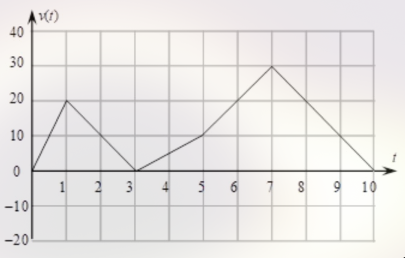
\includegraphics[width=0.5\textwidth]{Figures/Question-6.png}
 \end{center}
 If at $t = 0$ seconds, the position of the particle is at 20 meters, then at $t = 10$ seconds, its position is at 145 meters.\\

\textbf{Explanation}\\
The velocity-time graph can be divided into 5 sections, comprised of 4 triangles and 1 rectangle. To begin, calculate the areas of these 5 sections:
\begin{align*}
  A_1 &= \frac{1}{2} \cdot 3 \cdot 20 = 30\\
  A_2 &= \frac{1}{2} \cdot 2 \cdot 10 = 10\\
  A_3 &= \frac{1}{2} \cdot 4 \cdot 20 = 40\\
  A_4 &= \frac{1}{2} \cdot 1 \cdot 10 = 5\\
  A_5 &= 4 \cdot 10 = 40\\
\end{align*}
The total distance can be modeled by the following expression:
\begin{align*}
  x(0) + \int_0^t v(t) dt.
\end{align*}
Given that $x(0) = 20$ and $\int_0^t v(t) dt = A_1 + A_2 + A_3 + A_4 + A_5 = 125$, at $t = 10$:
\begin{align*}
  x(10) &= 20 + 125 = 145 \text{ meters}.\\
\end{align*}


\section*{Review}
\begin{enumerate}
  \item 
\end{enumerate}


\section*{Links to Other Notes}
\begin{itemize}
  \item \hyperref[]{}
\end{itemize}

\section*{Table of Contents}

\begin{itemize}
  \item \hyperref[toc]{TOC}
\end{itemize}

